\documentclass{beamer}
\usetheme{Berlin}
\usepackage{graphicx}
\usepackage[UKenglish]{isodate}
\usepackage{tikz}
\usepackage{pgfplots}
\pgfplotsset{compat=1.17}

\graphicspath{{./images/}}
\beamertemplatenavigationsymbolsempty

\title{Processor Simulator}
\author{George Herbert}
% \institute[University of Bristol, Bristol, U.K.]{University of Bristol\\Bristol, U.K.}
\date{\today}

\begin{document}

\begin{frame}
    \titlepage
\end{frame}

\section{Architecture}
\begin{frame}{High-Level Architecture Diagram}
    % 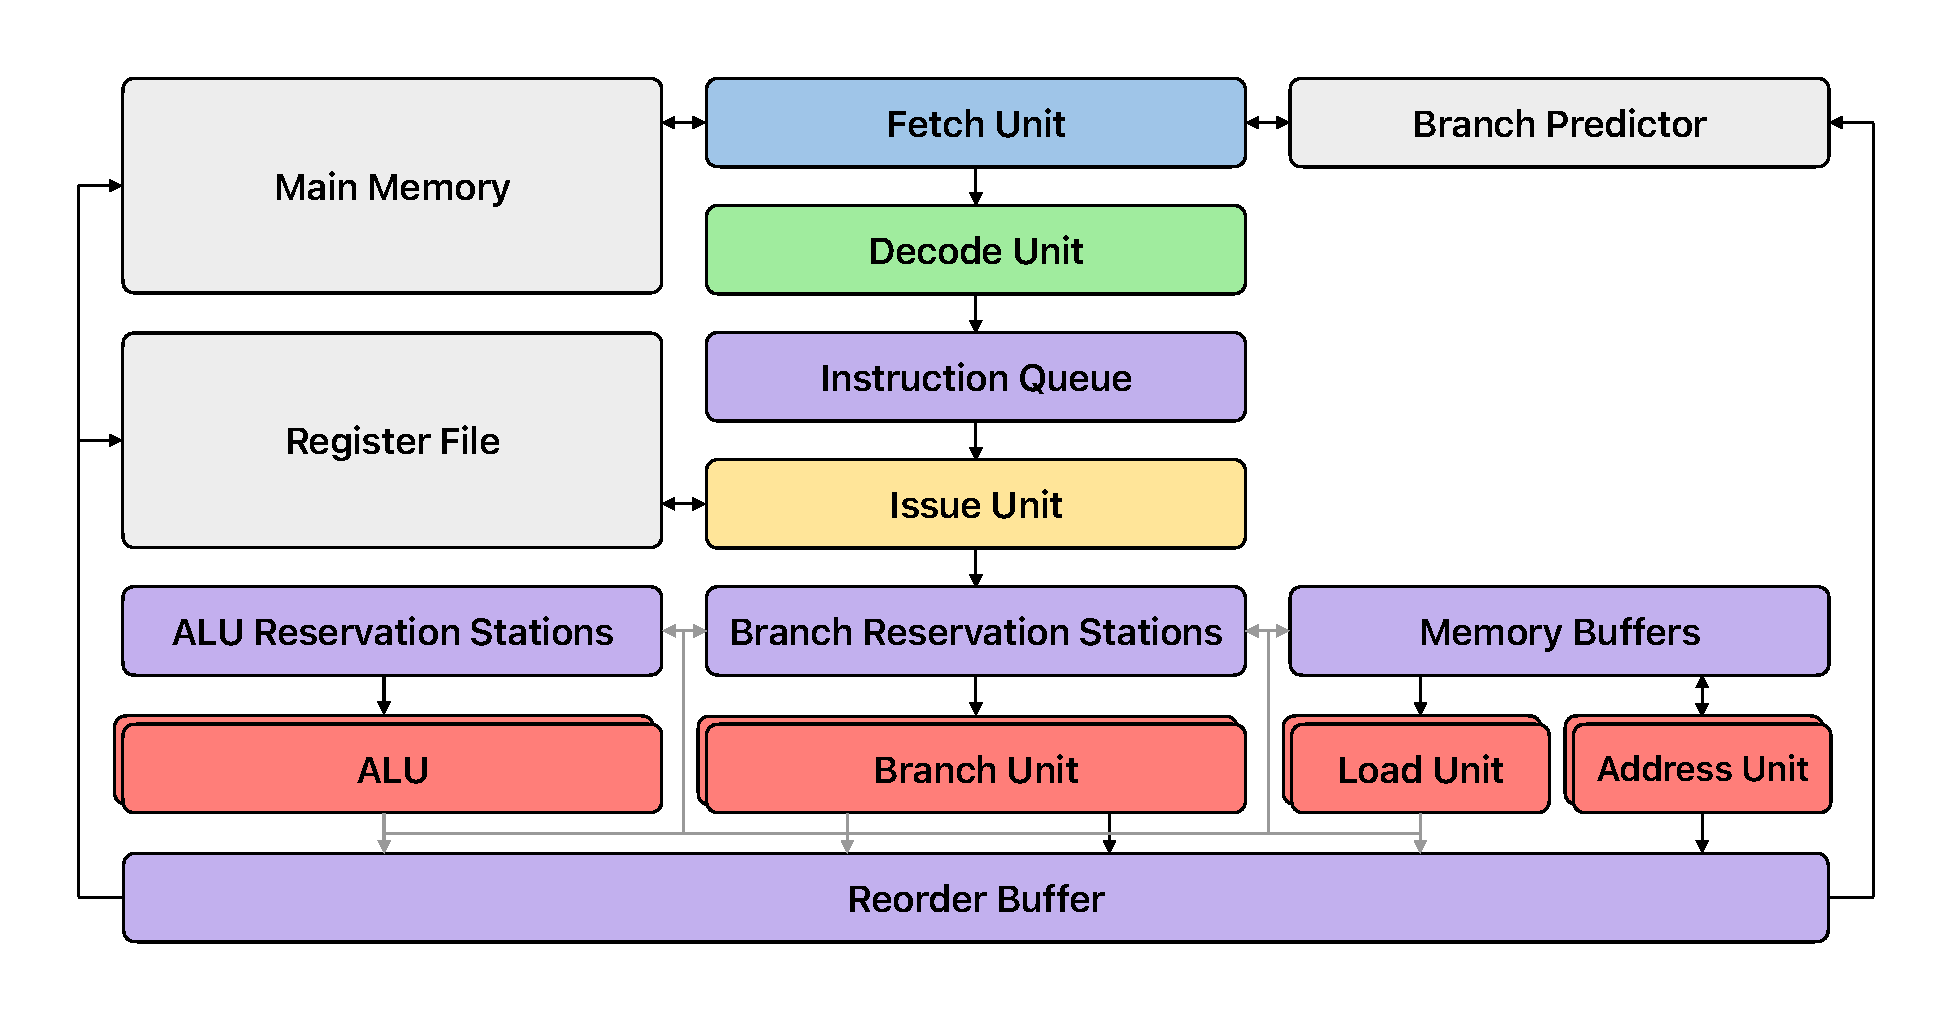
\includegraphics[width = \textwidth]{architecture.pdf}
\end{frame}

\begin{frame}{Feature Highlights}
    \begin{itemize}
        \item $n$-way superscalar        
        \item Speculative execution with a reorder buffer
        \item Dynamic branch prediction
        \item Out-of-order execution with Tomasulo's algorithm
        \item RV32I base integer instruction set
    \end{itemize}
\end{frame}

\begin{frame}{Configurable Components}
    \begin{itemize}
        \item Fetch/Decode/Issue width
        \item Commit width
        \item Number of ALUs, branch units, address units and load units
        \item Number of reservation stations and memory buffers
        \item Reorder buffer size
        \item Instruction queue size
        \item Branch target buffer size
        \item Execution cycles for each instruction
    \end{itemize}
\end{frame}

\section{Experiments}
\begin{frame}{Reorder Buffer Size}
    \onslide<1>{
        \begin{tikzpicture}[remember picture,overlay]
            \node[align=center, text width=\textwidth] at (current page.center) {
                \textbf{Hypothesis:} Increasing the reorder buffer size will enhance performance to a certain extent. However, the performance will plateau after reaching a certain point due to dependencies between instructions or bottlenecking elsewhere.
            };
        \end{tikzpicture}
    }
    \onslide<2>{
    \centering
    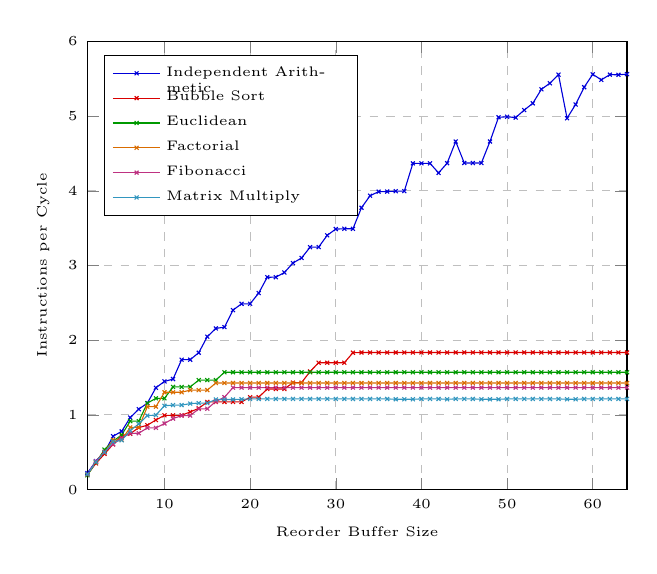
\begin{tikzpicture}
        \begin{axis}[
            xlabel={Reorder Buffer Size},
            ylabel={Instructions per Cycle},
            xmin=1, xmax=64,
            ymin=0,
            ymax=6,
        %   xtick={1,16,32,64,128},
            ytick={0,1,2,3,4,5,6},
            legend pos=north west,
            grid=major,
            ymajorgrids=true,
            xmajorgrids=true,
            grid style=dashed,
        %   grid style=dashed,
            tick label style={font=\tiny},
            label style={font=\tiny},
            legend style={font=\tiny, nodes={text width=2.25cm, align=left}}
        ]
        
        \addplot[
            color=blue!85!black,
            mark=x,
            mark options={scale=0.5},
        ] coordinates {
            (1, 0.22205) (2, 0.382546) (3, 0.50072) (4, 0.714969) (5, 0.780046) (6, 0.964965) (7, 1.077215) (8, 1.158408) (9, 1.363761) (10, 1.448703) (11, 1.479996) (12, 1.739495) (13, 1.739712) (14, 1.832784) (15, 2.04785) (16, 2.158107) (17, 2.17498) (18, 2.403075) (19, 2.487303) (20, 2.487303) (21, 2.63129) (22, 2.843213) (23, 2.843795) (24, 2.906185) (25, 3.032926) (26, 3.100535) (27, 3.245217) (28, 3.246732) (29, 3.404063) (30, 3.487713) (31, 3.491215) (32, 3.491215) (33, 3.773467) (34, 3.933541) (35, 3.988816) (36, 3.98996) (37, 3.994543) (38, 3.995691) (39, 4.367033) (40, 4.367033) (41, 4.367033) (42, 4.239256) (43, 4.369777) (44, 4.659631) (45, 4.372524) (46, 4.37115) (47, 4.372524) (48, 4.659631) (49, 4.983518) (50, 4.990671) (51, 4.97995) (52, 5.079985) (53, 5.170632) (54, 5.357858) (55, 5.439578) (56, 5.554712) (57, 4.971051) (58, 5.1553) (59, 5.386909) (60, 5.559153) (61, 5.484621) (62, 5.554712) (63, 5.552495) (64, 5.561375)
        };
        \addlegendentry{Independent Arithmetic}

        \addplot[
            color=red!85!black,
            mark=x,
            mark options={scale=0.5},
        ] coordinates {
            (1, 0.204633) (2, 0.351518) (3, 0.478745) (4, 0.606507) (5, 0.723326) (6, 0.747528) (7, 0.830574) (8, 0.862305) (9, 0.932868) (10, 0.994737) (11, 0.994746) (12, 0.994755) (13, 1.040155) (14, 1.088835) (15, 1.17406) (16, 1.17406) (17, 1.17406) (18, 1.17406) (19, 1.17406) (20, 1.237814) (21, 1.237814) (22, 1.347569) (23, 1.347601) (24, 1.347601) (25, 1.432238) (26, 1.432292) (27, 1.581266) (28, 1.699056) (29, 1.699081) (30, 1.699094) (31, 1.699107) (32, 1.832973) (33, 1.835866) (34, 1.835866) (35, 1.835866) (36, 1.835866) (37, 1.835866) (38, 1.835866) (39, 1.835866) (40, 1.835866) (41, 1.835866) (42, 1.835866) (43, 1.835866) (44, 1.835866) (45, 1.835866) (46, 1.835866) (47, 1.835866) (48, 1.835866) (49, 1.835866) (50, 1.835866) (51, 1.835866) (52, 1.835866) (53, 1.835866) (54, 1.835866) (55, 1.835866) (56, 1.835866) (57, 1.835866) (58, 1.835866) (59, 1.835866) (60, 1.835866) (61, 1.835866) (62, 1.835866) (63, 1.835866) (64, 1.835866)
        };
        \addlegendentry{Bubble Sort}
        
        \addplot[
            color=green!60!black,
            mark=x,
            mark options={scale=0.5},
        ] coordinates {
            (1, 0.192983) (2, 0.366659) (3, 0.536564) (4, 0.647021) (5, 0.733284) (6, 0.916575) (7, 0.916577) (8, 1.157723) (9, 1.222018) (10, 1.222018) (11, 1.374717) (12, 1.374717) (13, 1.374717) (14, 1.466336) (15, 1.466336) (16, 1.466336) (17, 1.571027) (18, 1.571027) (19, 1.571027) (20, 1.571027) (21, 1.571027) (22, 1.571027) (23, 1.571027) (24, 1.571027) (25, 1.571027) (26, 1.571027) (27, 1.571027) (28, 1.571027) (29, 1.571027) (30, 1.571027) (31, 1.571027) (32, 1.571027) (33, 1.571027) (34, 1.571027) (35, 1.571027) (36, 1.571027) (37, 1.571027) (38, 1.571027) (39, 1.571027) (40, 1.571027) (41, 1.571027) (42, 1.571027) (43, 1.571027) (44, 1.571027) (45, 1.571027) (46, 1.571027) (47, 1.571027) (48, 1.571027) (49, 1.571027) (50, 1.571027) (51, 1.571027) (52, 1.571027) (53, 1.571027) (54, 1.571027) (55, 1.571022) (56, 1.571022) (57, 1.571022) (58, 1.571022) (59, 1.571022) (60, 1.571022) (61, 1.571022) (62, 1.571022) (63, 1.571022) (64, 1.571022)
        };
        \addlegendentry{Euclidean}

        \addplot[
            color=orange!85!black,
            mark=x,
            mark options={scale=0.5},
        ] coordinates {
            (1, 0.204095) (2, 0.370383) (3, 0.500009) (4, 0.666579) (5, 0.66665) (6, 0.833183) (7, 0.83322) (8, 1.110634) (9, 1.110677) (10, 1.303601) (11, 1.303616) (12, 1.303616) (13, 1.332609) (14, 1.332609) (15, 1.332609) (16, 1.427625) (17, 1.427625) (18, 1.427625) (19, 1.427647) (20, 1.427647) (21, 1.427647) (22, 1.427647) (23, 1.427647) (24, 1.427647) (25, 1.427647) (26, 1.427647) (27, 1.427647) (28, 1.427647) (29, 1.427647) (30, 1.427647) (31, 1.427647) (32, 1.427647) (33, 1.427647) (34, 1.427647) (35, 1.427647) (36, 1.427647) (37, 1.427647) (38, 1.427647) (39, 1.427647) (40, 1.427647) (41, 1.427638) (42, 1.427638) (43, 1.427638) (44, 1.427638) (45, 1.427638) (46, 1.427638) (47, 1.427638) (48, 1.427638) (49, 1.427638) (50, 1.427638) (51, 1.427638) (52, 1.427638) (53, 1.427638) (54, 1.427638) (55, 1.427638) (56, 1.427638) (57, 1.427638) (58, 1.427638) (59, 1.427638) (60, 1.427638) (61, 1.427638) (62, 1.427638) (63, 1.427638) (64, 1.427638)

        };
        \addlegendentry{Factorial}

        \addplot[
            color=magenta!75!black,
            mark=x,
            mark options={scale=0.5},
        ] coordinates {
            (1, 0.206261) (2, 0.380152) (3, 0.508153) (4, 0.606204) (5, 0.690419) (6, 0.753103) (7, 0.755075) (8, 0.827116) (9, 0.827116) (10, 0.885561) (11, 0.95132) (12, 0.991402) (13, 0.991402) (14, 1.0806) (15, 1.082629) (16, 1.180143) (17, 1.237124) (18, 1.366114) (19, 1.366114) (20, 1.366114) (21, 1.366114) (22, 1.366114) (23, 1.366114) (24, 1.366114) (25, 1.366114) (26, 1.366114) (27, 1.366114) (28, 1.366114) (29, 1.366114) (30, 1.366114) (31, 1.366114) (32, 1.366114) (33, 1.366114) (34, 1.366114) (35, 1.366114) (36, 1.366114) (37, 1.366114) (38, 1.366114) (39, 1.366114) (40, 1.366114) (41, 1.366114) (42, 1.366114) (43, 1.366114) (44, 1.366114) (45, 1.366114) (46, 1.366114) (47, 1.366114) (48, 1.366114) (49, 1.366114) (50, 1.366114) (51, 1.366114) (52, 1.366114) (53, 1.366114) (54, 1.366114) (55, 1.366114) (56, 1.366114) (57, 1.366114) (58, 1.366114) (59, 1.366114) (60, 1.366114) (61, 1.366114) (62, 1.366114) (63, 1.366114) (64, 1.366114)
        };
        \addlegendentry{Fibonacci}

        \addplot[
            color=cyan!75!black,
            mark=x,
            mark options={scale=0.5},
        ] coordinates {
            (1, 0.206554) (2, 0.369505) (3, 0.498147) (4, 0.640211) (5, 0.660804) (6, 0.789958) (7, 0.880372) (8, 0.991322) (9, 0.998237) (10, 1.122679) (11, 1.131717) (12, 1.131726) (13, 1.151271) (14, 1.158412) (15, 1.158412) (16, 1.20652) (17, 1.20652) (18, 1.20652) (19, 1.209005) (20, 1.214324) (21, 1.214324) (22, 1.214324) (23, 1.214324) (24, 1.214324) (25, 1.214324) (26, 1.214324) (27, 1.214324) (28, 1.214324) (29, 1.214324) (30, 1.214324) (31, 1.214324) (32, 1.214324) (33, 1.214324) (34, 1.214324) (35, 1.214324) (36, 1.214324) (37, 1.20973) (38, 1.20973) (39, 1.20973) (40, 1.214324) (41, 1.214324) (42, 1.214324) (43, 1.20973) (44, 1.214324) (45, 1.214324) (46, 1.214324) (47, 1.20973) (48, 1.20973) (49, 1.20973) (50, 1.214324) (51, 1.214324) (52, 1.214324) (53, 1.214324) (54, 1.214314) (55, 1.214314) (56, 1.214314) (57, 1.20972) (58, 1.20972) (59, 1.214314) (60, 1.214314) (61, 1.214314) (62, 1.214314) (63, 1.214314) (64, 1.214314)
        };
        \addlegendentry{Matrix Multiply}
        \end{axis}
    \end{tikzpicture}
    }
    \onslide<3>{
        \begin{tikzpicture}[remember picture,overlay]
            \node[align=center, text width=\textwidth] at (current page.center) {
                \textbf{Outcome:} We broadly observe an increase in performance for all benchmarks as the reorder buffer size increases. The increase is most significant in the case of the arbitrary arithmetic benchmark since it has very few dependencies between instructions. When the reorder buffer size is one, the processor behaves as a single-issue in-order processor.
            };
        \end{tikzpicture}
    }
\end{frame}

\begin{frame}{Branch Prediction}
    \onslide<1>{
        \begin{tikzpicture}[remember picture,overlay]
            \node[align=center, text width=\textwidth] at (current page.center) {
                \textbf{Hypothesis:} Dynamic branch prediction will mispredict fewer branches than static branch prediction. Out of the dynamic branch predictors, a 2-bit saturating counter will mispredict fewer branches than a 1-bit saturating counter.
            };
        \end{tikzpicture}
    }
    \onslide<2>{
    \centering
    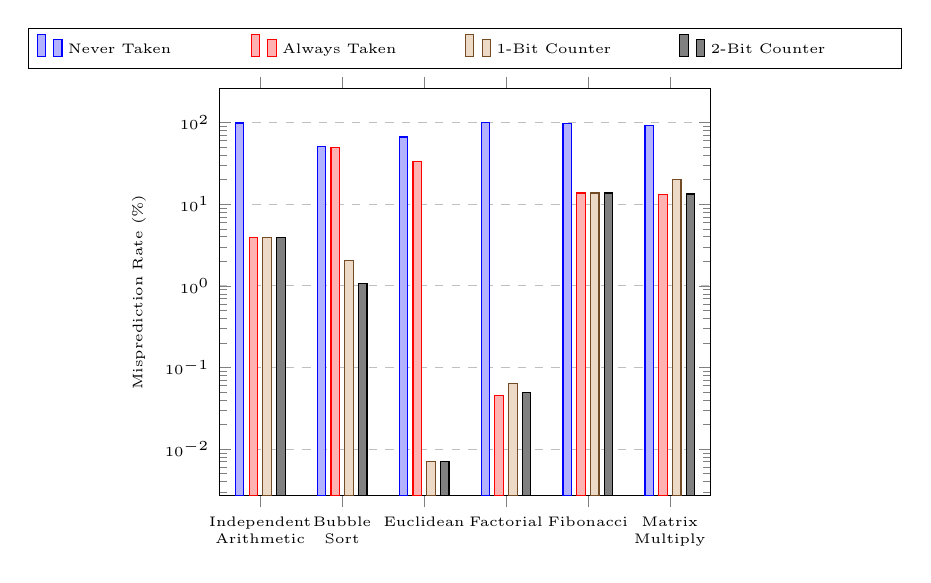
\begin{tikzpicture}
        \begin{axis}[
            ybar,
            ylabel={Misprediction Rate (\%)},
            xtick={1,2,3,4,5,6},
            xticklabels={
                {Independent\\Arithmetic},
                {Bubble\\Sort},
                {Euclidean},
                {Factorial},
                {Fibonacci},
                {Matrix\\Multiply}
            },
            xticklabel style = {font=\small},
            bar width=3pt,
            ymin=0,
            height = 6.75cm,
            ymajorgrids=true,
            grid style=dashed,
            tick label style={font=\tiny},
            label style={font=\tiny},
            x tick label style = {font=\tiny, align=center},
            legend style={font=\tiny, nodes={text width=2.25cm, align=left}, at={(0.5,1.15)}, anchor=north,legend columns=-1},
            ymode=log,
            log origin=infty,
          ]
 
          \addplot coordinates {
            (1, 99.029)
            (2, 50.980)
            (3, 66.668)
            (4, 99.978)
            (5, 98.039)
            (6, 93.303)
          };

          \addplot coordinates {
            (1, 3.883)
            (2, 49.049)
            (3, 33.337)
            (4, 0.045)
            (5, 13.725)
            (6, 13.311)
          };
      
          \addplot coordinates {
            (1, 3.883)
            (2, 2.028)
            (3, 0.007)
            (4, 0.063)
            (5, 13.725)
            (6, 19.906)
          };

          \addplot coordinates {
            (1, 3.883)
            (2, 1.077)
            (3, 0.007)
            (4, 0.050)
            (5, 13.725)
            (6, 13.343)
          };

          \legend{Never Taken, Always Taken, 1-Bit Counter, 2-Bit Counter}
        \end{axis}
      \end{tikzpicture}
    }
    \onslide<3>{
        \begin{tikzpicture}[remember picture,overlay]
            \node[align=center, text width=\textwidth] at (current page.center) {
                \textbf{Outcome:} We observe the 2-bit saturating counter to outperform the 1-bit saturating counter in all benchmarks. We believe this is because the 1-bit saturating counter causes most conditional branches to mispredict twice (e.g. for loop-closing branches, we mispredict once when we do not take it, then again the next time we take it). Interestingly, in some benchmarks, the always-taken predictor performs equally as well as the 2-bit saturating counter. In the case of the independent arithmetic benchmark, this is because there is only a single loop in the benchmark, which we iterate over a fixed number of times.
            };
        \end{tikzpicture}
    }
\end{frame}

\begin{frame}{Fetch/Decode/Issue/Commit Width}
    \onslide<1>{
        \begin{tikzpicture}[remember picture,overlay]
            \node[align=center, text width=\textwidth] at (current page.center) {
                \textbf{Hypothesis:} Increasing the fetch/decode/issue/commit width will enhance performance to a certain extent. However, the performance will plateau after reaching a certain point due to dependencies between instructions, the presence of branches, or bottlenecking elsewhere.
            };
        \end{tikzpicture}
    }
    \onslide<2>{
    \centering
    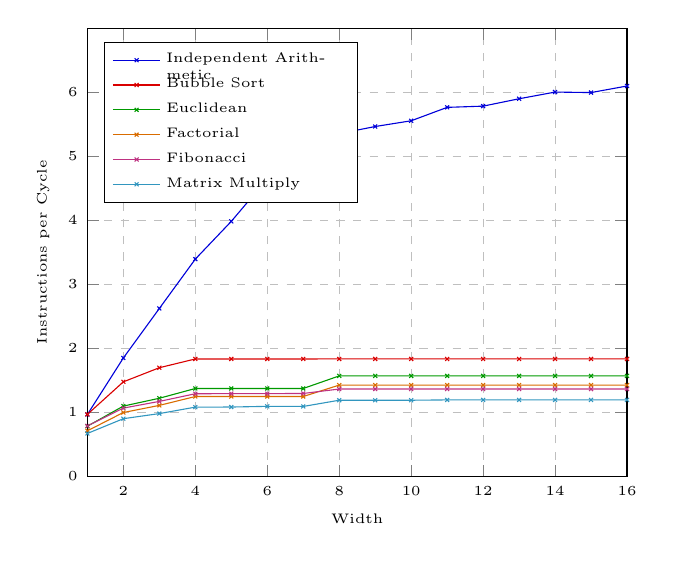
\begin{tikzpicture}
        \begin{axis}[
            xlabel={Width},
            ylabel={Instructions per Cycle},
            xmin=1, xmax=16,
            ymin=0,
            ymax=7,
        %   xtick={1,16,32,64,128},
            ytick={0,1,2,3,4,5,6},
            legend pos=north west,
            grid=major,
            ymajorgrids=true,
            xmajorgrids=true,
            grid style=dashed,
        %   grid style=dashed,
            tick label style={font=\tiny},
            label style={font=\tiny},
            legend style={font=\tiny, nodes={text width=2.25cm, align=left}}
        ]
        
        \addplot[
            color=blue!85!black,
            mark=x,
            mark options={scale=0.5},
        ] coordinates {
            (1, 0.969201) (2, 1.851324) (3, 2.623845) (4, 3.394923) (5, 3.984245) (6, 4.647177) (7, 5.134367) (8, 5.353734) (9, 5.465226) (10, 5.554712) (11, 5.764194) (12, 5.783368) (13, 5.898643) (14, 6.003021) (15, 5.995259) (16, 6.097764)

        };
        \addlegendentry{Independent Arithmetic}

        \addplot[
            color=red!85!black,
            mark=x,
            mark options={scale=0.5},
        ] coordinates {
            (1, 0.970474) (2, 1.478469) (3, 1.698902) (4, 1.835747) (5, 1.835806) (6, 1.835851) (7, 1.835851) (8, 1.835866) (9, 1.835881) (10, 1.835881) (11, 1.835881) (12, 1.835866) (13, 1.835866) (14, 1.835866) (15, 1.835866) (16, 1.835866)
        };
        \addlegendentry{Bubble Sort}
        
        \addplot[
            color=green!60!black,
            mark=x,
            mark options={scale=0.5},
        ] coordinates {
            (1, 0.785619) (2, 1.099813) (3, 1.221998) (4, 1.374688) (5, 1.374709) (6, 1.374717) (7, 1.374717) (8, 1.571011) (9, 1.571011) (10, 1.571011) (11, 1.571011) (12, 1.571011) (13, 1.571011) (14, 1.571011) (15, 1.571011) (16, 1.571011)
        };
        \addlegendentry{Euclidean}

        \addplot[
            color=orange!85!black,
            mark=x,
            mark options={scale=0.5},
        ] coordinates {
            (1, 0.714135) (2, 0.99965) (3, 1.11065) (4, 1.249309) (5, 1.249373) (6, 1.249376) (7, 1.2494) (8, 1.427559) (9, 1.427559) (10, 1.42759) (11, 1.42759) (12, 1.42759) (13, 1.42759) (14, 1.427594) (15, 1.427594) (16, 1.427594)
        };
        \addlegendentry{Factorial}

        \addplot[
            color=magenta!75!black,
            mark=x,
            mark options={scale=0.5},
        ] coordinates {
            (1, 0.790267) (2, 1.068582) (3, 1.17294) (4, 1.292601) (5, 1.294052) (6, 1.294052) (7, 1.296963) (8, 1.366114) (9, 1.366114) (10, 1.366114) (11, 1.366114) (12, 1.366114) (13, 1.366114) (14, 1.366114) (15, 1.366114) (16, 1.366114)
        };
        \addlegendentry{Fibonacci}

        \addplot[
            color=cyan!75!black,
            mark=x,
            mark options={scale=0.5},
        ] coordinates {
            (1, 0.672568) (2, 0.903071) (3, 0.982551) (4, 1.083541) (5, 1.085019) (6, 1.095817) (7, 1.094134) (8, 1.19129) (9, 1.191122) (10, 1.191171) (11, 1.196334) (12, 1.196334) (13, 1.196334) (14, 1.196324) (15, 1.196324) (16, 1.196324)
        };
        \addlegendentry{Matrix Multiply}
        \end{axis}
    \end{tikzpicture}
    }
    \onslide<3>{
        \begin{tikzpicture}[remember picture,overlay]
            \node[align=center, text width=\textwidth] at (current page.center) {
                \textbf{Outcome:} We observe a consistent increase in performance for all benchmarks as the width increases. The increase is most significant in the case of the arbitrary arithmetic benchmark since it has very few dependencies between instructions and very few branches. The width of the pipeline serves as an upper bound on the IPC because we cannot complete more instructions in any given cycle than the width of the pipeline.
            };
        \end{tikzpicture}
    }
\end{frame}

\end{document}
